\subsection{Bubble Game (start)} % (fold)
\label{sub:bubble_game_start_}

The bubble game has ten floating bubbles for the user to `pop'. Each bubble is a sprite, which gives it a location on the screen and a movement vector. When the program run the bubbles move in random directions, reappearing at a new random location if they go off the screen.

\begin{figure}[h]
   \centering
   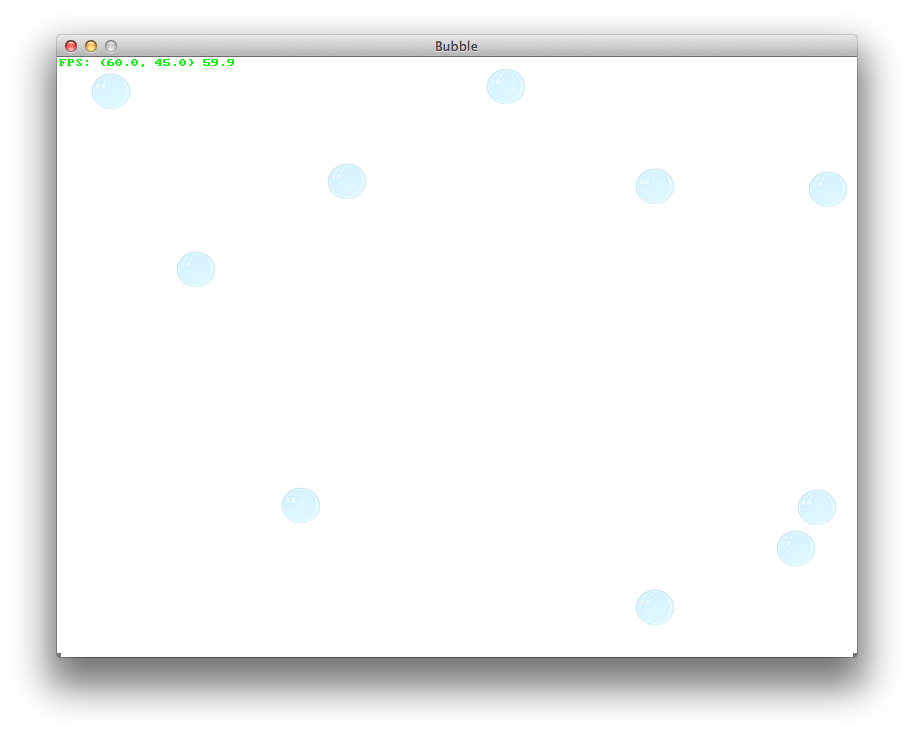
\includegraphics[width=0.8\textwidth]{./topics/type-decl/examples/Bubbles.png} 
   \caption{Example execution of the Bubbles program}
   \label{fig:bubbles-img}
\end{figure}

\clearpage

\cppsection{\ccode{cpplst:bubble-game}{Starting code for a Bubble Game in C++, continues in \lref{cpplst:bubble-game1} }{topics/arrays/examples/bubble-game.c}}

\cppsection{\ccode{cpplst:bubble-game1}{Starting code for a Bubble Game in C++ (continued)}{topics/arrays/examples/bubble-game1.c}}

\passection{\pascode{plst:bubble-game}{Starting code for a Bubble Game in Pascal, continues in \lref{plst:bubble-game1} }{topics/arrays/examples/BubbleGame.pas}}

\passection{\pascode{plst:bubble-game1}{Starting code for a Bubble Game in Pascal (continued)}{topics/arrays/examples/BubbleGame1.pas}}


% subsection bubble_game_start_ (end)